\section{Security of Availability and Validity}


\begin{theorem}[Availability]
Assuming the Merkle tree constructed from collision resistant hash functions and a block in GRANDPA can be finalized with at least $2f+1$ votes, then the availability protocol is secure.
\end{theorem}

\begin{proof}
Assume that an unavailable block is finalized. It means that this finalized block includes a block header of which at most $f$ honest validators has the correct erasure code piece (See Definition \ref{def:unavail}). If this block is finalized, it means that either
\begin{itemize}
    \item not all honest validator who do not have the erasure code piece announce the unavailability. If they would announce it, since their number is at least $2f+1 - f =f+1$ (i.e., honest parties - honest parties who do not have the erasure code), the other honest parties do not finalize it and malicious parties do not have enough number to finalize it. Therefore, we can assume that there is at least one honest party who do not announce the unavailability of its erasure code in this case, because he thinks that he has one but actually it is not correct. If there exists one honest party who has incorrect erasure code, but having the proof that it is correct (provided by parachain validators), then it means that the collision resistance assumption of Merkle tree is broken. 
    
    \item or  $f+1$ parties announce unavailability means that GRANDPA finalized the block with at most $2f$  parties. So, this implies that the security of GRANDPA is broken by finalizing a block with less than $2f+1$ votes.
\end{itemize}

Since the GRANDPA is secure and the Merkle tree is collision resistant, the unavailability protocol is secure.
\end{proof}

\begin{theorem}[Validity]
\label{thm:valid}
Assuming that the availability protocol is secure, the signature scheme is EF-CMA secure, the hash function $H$ in Conditions (\ref{cond:time}) and  (\ref{cond:equiv}) is a random oracle, the PoV protocol is secure and correct (Definition \ref{def:pob}), the VRF is secure and a block in GRANDPA can be finalized with at least $2f+1$ votes then the invalid block is finalized in the relay chain with  the probability less than risk probability.
\end{theorem}

\begin{proof}(Sketch)
TODO: Security reduction, Rewrite the security arguments


If there is one honest $PV$ and there is not any $f+1$ unavailability report, then at least $2f$ of the honest parties has the piece. It means that $PV$ can collect all the pieces from the honest parties in order to reconstruct the blob and check its validity. Therefore, if there is at least one honest party in $PV$, it can detect the invalidity and announces it. In the end, we will have more than $f$ invalidity signatures since the other parties also check invalidity after seeing the signature saying that the block is invalid.

Therefore, all parachain validators have to be malicious not to be caught. 
If there is at least one honest validators who is assigned for an extra validity check with either of the conditions, then the same case happens as having at least one honest parachain validator. Therefore, an invalid block cannot be detected (the attack succeeds) if all parachain validators are malicious and all extra check validators are malicious as well. 

Remark that the extra check conditions (\ref{cond:mod}) and (\ref{cond:time})  with $\tau = 0$ and (\ref{cond:equiv}) and (\ref{cond:modequiv}) guarantees that the expected number of checks by parachain validators and the extra check validators is $\vcheck$. %In addition to this, the selection mechanism of parachain and extra check validators  guarantees with a overwhelming probability that each validator is responsible from only one parachain as an either extra-check validator or parachain validator. 
Therefore, we can consider that the parachain validator and extra-validator selection mechanism actually randomly samples $\vcheck$ validators for each parachain. So, the probability of all selected validators for a particular parachain being malicious is bounded by $(\frac{1}{3})^{\vcheck}$. See \ref{lem:permutation} for the details.

\end{proof}



\begin{theorem}\label{thm:vcheckmal}
Given that $\vcheck$ malicious validators are eligible to check the validity of a block header, the invalidity attack is bounded by the probability  $\exp(-\frac{2}{3}(\mu+r))$ if $\mu + r < n/m$ and the probability $\exp(-\frac{2n}{3m})$ if $\mu + r \geq n/m$.
\end{theorem}

\begin{proof}

Below, we give the probability of any validator being in conditions (\ref{cond:mod}), (\ref{cond:time}), (\ref{cond:modequiv}), (\ref{cond:equiv}):

$$\Pr[\text{Cond. (\ref{cond:mod})}] = \Pr[\text{Cond. (\ref{cond:modequiv})}] = p_{vrf} = \frac{1}{m}$$
$$\Pr[\text{Cond. (\ref{cond:time}) at time } \tau] = p_\tau =  \frac{\mu'}{n - nc} + \tau $$
$$\Pr[\text{Cond. (\ref{cond:equiv}) }] = \frac{\mu'}{n - nc} $$


We assume that $|\pv| = \frac{n}{m}$.  The number of $\vcheck-|\pv| = \mu + r$ malicious validators can be selected for the extra check with the following cases:

\begin{enumerate}
    
    \item $\mu + r \geq \frac{n}{m}$ and at least $\mu + r$ malicious validators are in condition (\ref{cond:mod}) and condition (\ref{cond:time}) until the time $\tau_k$ for the parachain whose validators are malicious. The attack probability is highest if at least $\mu + r$
    malicious validators are in (\ref{cond:mod}). In this case, the attack succeeds if no honest validator satisfies the condition (\ref{cond:mod}) 
    
    
    \begin{align}\label{eq:attack2}
        \Pr[\mathsf{attack1}] &= (1-\frac{1}{m})^{2n/3} <  e^{-2n/3m} \nonumber
    \end{align}
    
    
    \item $\mu+r < \frac{n}{m}$ and at least $\mu' = \mu+r$ malicious validators are in condition (\ref{cond:time}) until the time $\tau_k$. For simplicity, we divide time in discrete values $[\tau_0 = 0, \tau_1 =u, \tau_2 = 2u, ..., \tau_k = ku]$. $\tau_k$ can be computed by malicious validators before the validation process begins. The probability of this attack is the following
    
    \begin{align}
        \Pr[\mathsf{attack2}] &= \prod_{i = 0}^k(1-p_{\tau_i})^{\frac{2n}{3}} \nonumber\\
        &\leq  \prod_{i = 0}^k (1 - \frac{\mu'+\tau_in(1-c)}{n(1-c)})^{\frac{2n}{3}} \nonumber\\
        &=  \exp(\sum_{i = 0}^k -\frac{2}{3}\frac{\mu' + \tau_in(1-c)}{1-c}) \nonumber\\
        & = \exp(-2/3(\frac{(k+1)\mu'}{1-m/n}+ nu\frac{k(k+1)}{2})\nonumber
    \end{align}
    Remark that $\Pr[\mathsf{attack3}]$ is maximum when $k = 0$. When $k = 0$, $\Pr[\mathsf{attack3}] \leq \exp(-\frac{2\mu' n}{3(n-m)}) \leq \exp(-\frac{2}{3}(\mu + r))$.
    
    
    \item This case considers equivocation: Here, we can assume that the adversary knows who satisfies the condition (\ref{cond:mod}) and (\ref{cond:time}) since if the malicious validator is the block producer, he first produces the block and sees who validates this block. If no honest validator checks it with condition (\ref{cond:mod}), he equivocates it. When this happens, the attack succeeds if no honest party satisfies the condition (\ref{cond:modequiv}) or (\ref{cond:equiv}). Hence,
    the probability of attack 4 is
    
    \begin{align}
    \Pr[\mathsf{attack} 4] &= \Pr[\text{no honest check in  cond. (\ref{cond:equiv}) and (\ref{cond:modequiv})}]\nonumber \\ 
							&\leq \Pr[\mathsf{attack1}](1-\frac{\mu'}{n-nc)}) ^{\frac{2}{3}n} \nonumber\\
				            &\leq \exp({-2/3(\frac{n}{m}+\mu + r)}) \nonumber
    \end{align}
\end{enumerate}	
    % \item  In this attack, the adversary equivocates and it does it when $\mu'> n/m$ and there are $n/m$ malicious adversaries satisfying the condition (\ref{cond:mod}). we can assume that the adversary knows who satisfies the condition (\ref{cond:mod}) since if the malicious validator is the block producer, he first produces the block and sees who validates this block. If no honest validator checks it, he equivocates it with a block where at least $n/m$ malicious validators satisfies the condition (\ref{cond:modequiv}). Then, the attack succeeds if no honest party satisfies the condition (\ref{cond:equiv}). 
    % The probability of attack 3 is
    
    % \begin{align}
    % \Pr[\mathsf{attack}3] &= \Pr[\text{no honest check in  cond. (\ref{cond:equiv})}]\nonumber \\ 
				% 					   &\leq (1-\frac{\mu'}{n-nc)}) ^{\frac{2}{3}n} \nonumber\\
				% 					   &\leq e^{-2/3(\frac{\mu'}{1-c})} \nonumber
    % \end{align}
    
    





%
%Therefore, the attack probability is $\Pr[\mathsf{attack1}]+\Pr[\mathsf{attack2}]+\Pr[\mathsf{attack}3]$.



%Here, we consider $r_a = 0$ to compute the maximum attack probability and $c_f' = \lceil r_f \rceil$. We do not take $r_f = 0$, because we assume that there is always at least one fisherman.


%a parachain validator does not know who are the extra-check validators except the malicious validators if they are assigned to extra check. This comes from the VRF security. So , since $H$ is a random oracle, $B$ is derived from a uniform distribution between $[0,1]$. Therefore, the probability of a validator is assigned to be an investigator at time $\tau$ given that not enough validity check (i.e., $|\mathcal{I}| < \vcheck$) is done before $\tau$ is:

%$$p_{\tau} = \frac{\vcheck - |\pv|}{|\V|-|\pv|}+\tau  = \frac{1+\lceil \runav + \rinv \rceil}{n-nc}+ \tau$$

%assuming that $|PV| = nc$ where $c \in (0,1)$.

%Remark that when $\tau$ increases meaning that when the time increases without having sufficient validity check, $p_{\tau}$ increases and reaches 1 at some time. For simplicity, we divide time in discrete values $[\tau_0 = 0, \tau_1 =\mu', \tau_2 = 2\mu', ..., \tau_k = k\mu']$ where $k\mu'$ is the time when the number of malicious parties in $\mathcal{I}$ is $\vcheck$. This time can be computed by malicious validators before the validation process begins. In any case, the only way not to be caught is not to have any honest extra-check validator until $k\mu'$. The probability of this is the following given that  the number of malicious parties in $\mathcal{I}$ is $\vcheck$:

%\begin{align}
% \Pr[\mathsf{attack} = 1] = \prod_{i = 0}^k(1-p_{\tau_i})^{2f+1} \leq (1-p_{\tau_0})^{2f+1} &\leq (1-\frac{1+c'_f}{n(1-c)}) ^{\frac{2}{3}n} \nonumber \\
%& \leq e^{-2/3\frac{1+c_f}{1-c}} \nonumber
%\end{align}
%Here, we consider $r_a = 0$ to compute the maximum attack probability and $c_f' = \lceil r_f \rceil$. We do not take $r_f = 0$, because we assume that there is always at least one fisherman.



\end{proof}


\section{Practical Results}

As it can be seen from the proof of theorem \ref{thm:valid}, malicious validators can attack the validity protocol with probability $(\frac{1}{3})^{\vcheck}$. Remember that $\vcheck = |\pv| + \mu + r$ where $r = \lceil r_a + r_f \rceil$. If we assume that parachain validators change in every $x$ minutes, the malicious parties needs to wait $x3^{\vcheck}$ minutes in order to succeed the attack. For example, if $x = 5$ minutes, then the total time for an attack for each $\vcheck$ is given in Figure \ref{fig:totaltime}:


\begin{figure}[h]\centering
	  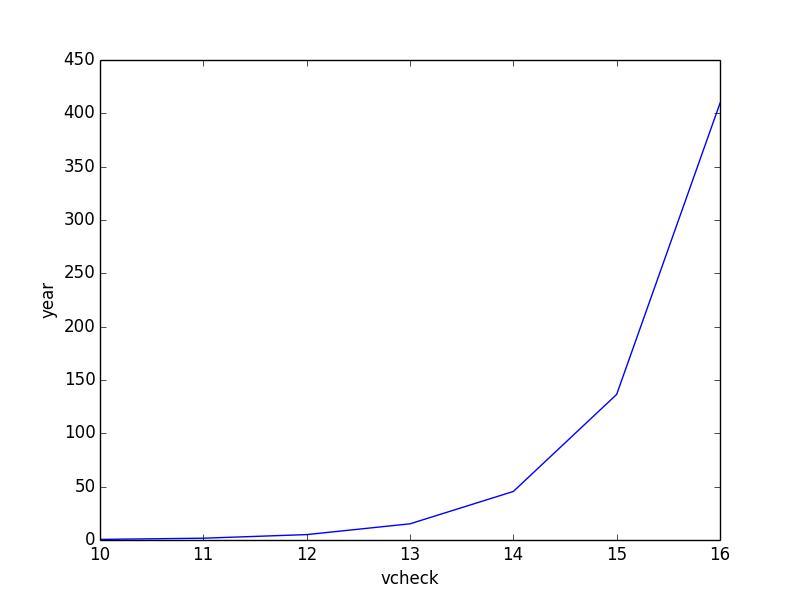
\includegraphics[width=10cm]{images/year.png}
	  \caption{It shows the waiting time for an adversary for a successful attack given that every parachain validators changes every 5 minutes}
	  \label{fig:totaltime}
\end{figure}

As it can be seen,  if $\vcheck$ is more than 14, the adversary needs to wait more than 50 years for the attack. Therefore, in terms of security, it is important to have  minimum $\vcheck$ validators.

\paragraph{The parameter $\mu$:} The possible $\mu$ (minimum number of extra check) values:

\begin{itemize}
    \item If $\mu = 0$, then $|pv| = 14$ in order to make sure that minimum $\vcheck$ is always equal to $14$. Given that $|pv| = n/m$ where $m$ is the number of parachain validators $n = 14 * m$. 
    
    \item If $\mu > 0$, then $|pv| < 14$. It means that we need less validators for the security than in the case where $\mu = 0$. Less validators imply less network delay and less network delay implies more secure BABE. On the other hand, if $\mu$ increases, it means that more validators need to reconstruct a blob in order to check the validity. So, validators need to do more work. In terms of scalability of the relay chain, we need to decide $\mu$. 
\end{itemize}
As rule of thumb, if we don't care about the number of validators as far as it is not the maximum  number of validators ($N$) that Polkadot can handle, then if $14 * m < N$, $\mu = 0$. Otherwise, $\mu = 14 -N/m$. 

Another disadvantage of having $\mu = 0$ is that parachain validators have a less risky attack  when all of them are malicious. Imagine a parachain with a few collators. We can assume that they may be malicious and collaborate with the malicious validators. In this case, the validators will not have any report. So, there will be 0 extra check. As soon as all parachain validators are malicious in this malicious parachain, they can add invalid block headers and cannot be caught. The security argument says here that they need to wait around 50 years for this, so the attack is not possible. However, in the real life, since the attack does not have any risk, the collators can bribe parachain validators with their stake and parachain validators validate an invalid blob.


Theorem \ref{thm:vcheckmal} gives the risk that  malicious validators take at  when they put an invalid report.  If $\mu + r \leq n/m$, the invalid block will not be detected with probability $\exp(-\frac{2}{3}(\mu+r))$. In the worst case scenario, if no report is received then the attack probability is $\exp(-\frac{2}{3}(\mu))$. We give in Figure \ref{fig:mu} that the probability of a successful attack in the case of $\vcheck$ malicious validators are selected. As it can be seen in Figure \ref{fig:mu}, their risk is exponentially increasing when $\mu$ increases. In order to make the risk close to 0 even if no report received, $\mu$ should be greater than $4$.

\begin{figure}[h]\centering
	  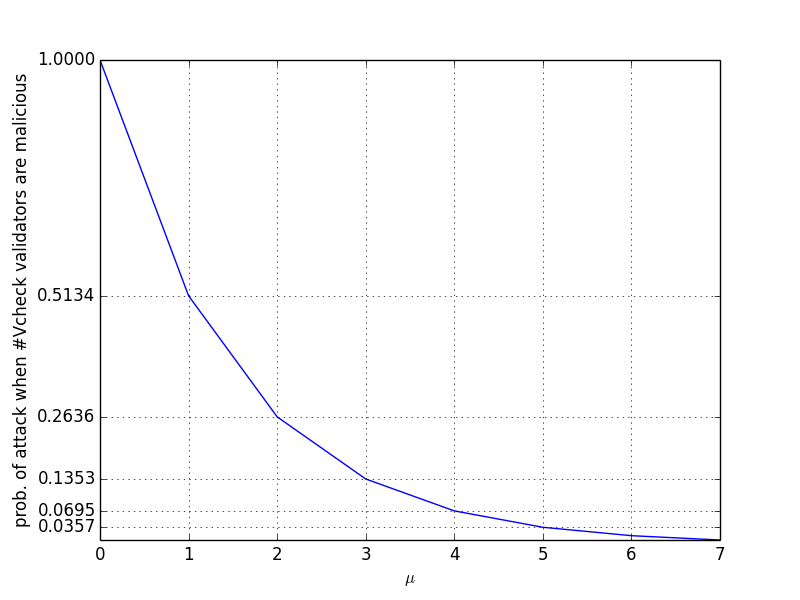
\includegraphics[width=12cm]{images/muval.png}
	  \caption{The risk of malicious validators when they attack even if $\vcheck$ validators are malicious}
	  \label{fig:mu}
\end{figure}

\paragraph{Fisherman and Collator Reports:} In the validity scheme, we rely on the invalidity reports of fishermen and  unavailability reports of collators to find the parameter $ \vcheck $. However, we need to bound $\vcheck$ so that these reports do not make too many validators to check the validity. Let us call this bound $\mu_{max}$ (i.e, $\mu + \lceil r_f + r_a \rceil \leq \mu_{max}$). This bound is necessary because regular malicious reports can slow down the process easily. 

When a fisherman sends a report of invalidity, but later on it is found to be valid, the fisherman is slashed. Therefore, the reliability of a fisherman report can be measured by how much it is staked. 
Considering this, $r_f$ can be computed as follows:

$$r_f = \frac{\sum_{i}\mathsf{stake}_{f_i}}{v_{gain}}$$

Here, $\mathsf{stake}_{f_i}$ is the stake that a fisherman $f_i$ puts for this report and $v_{gain}$ is the DOT value that a validator receives in each block. In a nutshell, a fisherman needs to stake at least the same amount that the validator earns for each block in order to make a validator to execute an extra validity check. If the fisherman report is not valid, then the fisherman pays for this extra check. So, a malicious fisherman has to spend $\mu_{max} v_{gain}$ for a report to slow down the validator network. We believe that this model discourages fishermen to send false reports. 

However, we cannot measure the reliability of unavailability reports as fisherman's reports since it is not possible to show the correctness or incorrectness of any unavailability reports. Malicious collators do not lose anything by just sending fake unavailability reports. In order to solve this issue, we assign a parameter $\alpha \in (0,1)$ for a parachain that defines the proportion of honest collator assumption. Depending on $\alpha$, we have define $r_a$ for two cases:
\begin{itemize}
    \item if $\alpha > 1/2$, $r_a = \mu_{max}^{x/\alpha}$ 
    
        \[   
    r_a(x)= 
     \begin{cases}
       \mu_{max}^{x/\alpha} & \text{if } x \leq \alpha \\
       \mu_{max} &\text{otherwise} \\ 
     \end{cases}
\]  
    
    where 
    $$x = \frac{\text{total unavailability reports}}{\text{all collators}} = \frac{\sum_{c_i \in C_P}st_{c_i}}{|C_P|}.$$
    
    Here, $st_{c_i}\in \{0,1\}$ and it is 0 if the block is available. Otherwise, it is 1. The reason of using a function such as $\mu_{max}^{x/\alpha}$ is to make sure that we have extra checks close to maximum check only if the number of unavailability reports are close to the number of honest collator assumption. Thanks to this, if the number of honest collators are majority, the malicious collators who want to slow down Polkadot cannot achieve to make always maximum number of checks with only unavailability reports. In general, these type of parachains can be investigated by fishermen as far as the blocks are available to honest collators. Therefore, we expect that if there is any invalid block, the fishermen catch it and send a report. If the blocks are unavailable to honest collators (so fishermen too), validators checks the invalidity with the maximum capacity.  
    
    \item if $\alpha < 1/2$, then it is critical to give more importance to the unavailability reports from this parachain. Therefore, we use the following linear function:
    
    \[   
    r_a(x)= 
     \begin{cases}
       \mu_{max}\frac{x}{\alpha} & \text{if } x \leq \alpha \\
       \mu_{max} &\text{otherwise} \\ 
     \end{cases}
\]  
\end{itemize}

So, $\mu' = \mu + \lceil r_a + r_f \rceil$ if $\mu + \lceil r_a + r_f \rceil \leq \mu_{max}$. Otherwise, $\mu' = \mu_{max}$.


\paragraph{The parameter $\mu_{max}$:} Given the fact that we have maximum number of extra checks when there are many invalidity or unavailability  reports, the parameter $\mu_{max}$ needs to be big enough so that the probability of having at least one honest extra check is almost 1.
This probability can be bounded by $1-(\frac{1}{3})^{\mu_{max}}$. Therefore, we can have $\mu_{max} = 15$.

In Figure \ref{fig:ra}, we compute the number of extra checks required depending on the $\alpha$-parameter of a parachain. As it can be seen, the parachain that we trust less requires more extra-checks. The parachain where we assume honest majority reaches the maximum check when the unavailability reports are close to the number of honest collators.  


\begin{figure}[h]\centering
	  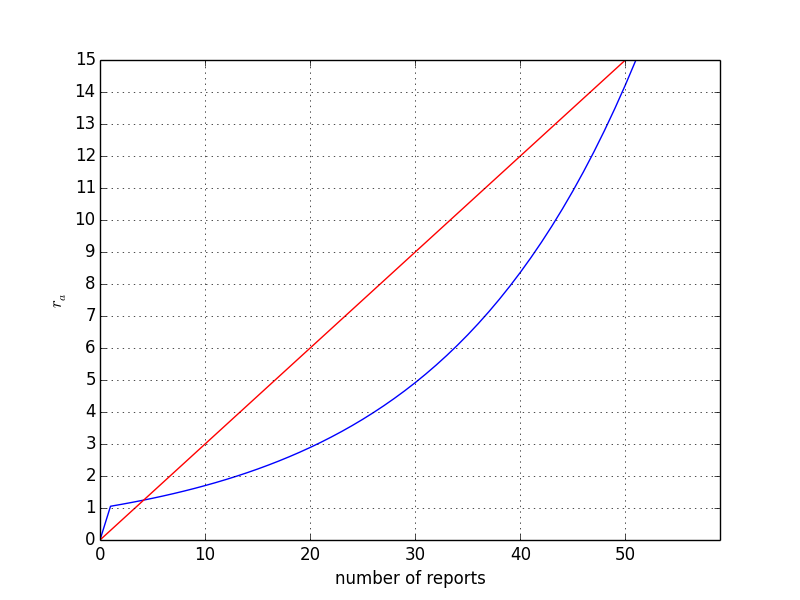
\includegraphics[width=10cm]{images/ra.png}
	  \caption{The red and blue graph shows the number of required extra checks when $\alpha \leq 1/2$ and $\alpha > 1/2$. Here, we assume that the total number of collators are 100.}
	  \label{fig:ra}
\end{figure}

